\section{Introduction}

A \emph{process} is defined as a series of inter-related events that involve multiple entities and lead to an end result. Product manufacturing, economical developments, and various phenomena in life and social sciences can all be viewed as types of processes. Processes are complicated objects; consider for example the biological process of ATP synthesis described in Figure~\ref{fig:process}. This process involves 12 entities and 8 events. Additionally, it describes relations between events and entities, and the relationship between events (e.g., the second occurrence of the event \textit{`enter'}, causes the event \textit{`changing'}). 

\begin{figure*}[ht]
\centering
\fbox{ 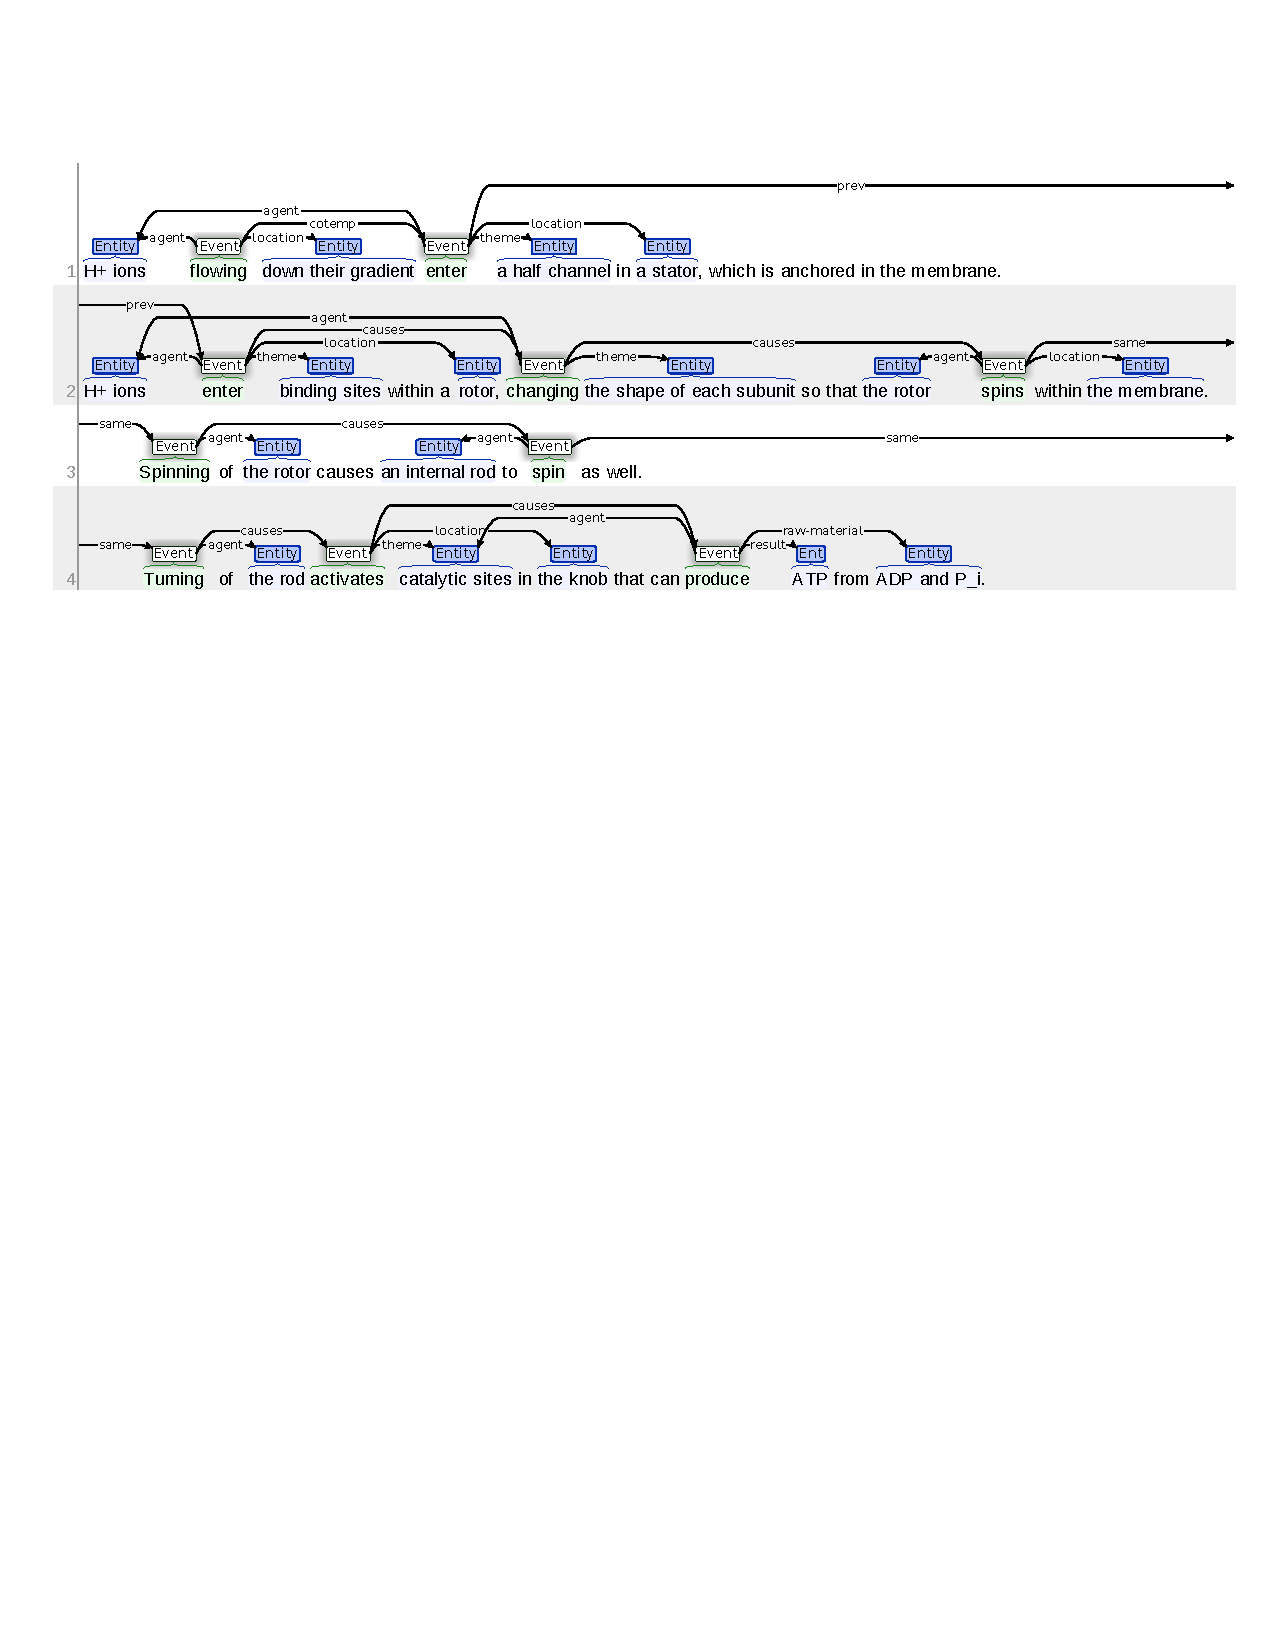
\includegraphics[width=0.98\textwidth]{figures/process5}}
\caption{Partial annotation of the ATP synthesis process. Most of the semantic roles have been removed for simplicity.}
\label{fig:process}
\end{figure*}

Automatically extracting the structure of processes from text is crucial for applications that require reasoning, such as non-factoid QA. For instance, answering a question on ATP synthesis, such as \emph{``How do H+ ions contribute to the production of ATP?"} requires a structure that links \emph{H+ ions} (Figure~\ref{fig:process}, sentence 1) to \emph{ATP} (Figure~\ref{fig:process}, sentence 4) through a sequence of intermediate events. Such \emph{``How?"} questions are common on FAQ websites \cite{Surdeanu:2011}, which further supports the importance of process extraction.

%Automatically extracting the structure of processes from text is crucial for applications such as non-factoid QA. A human reading the example paragraph can answer questions such as:
%\begin{enumerate}[itemsep=0pt,topsep=0pt] 
%\footnotesize \emph{How do H+ ions contribute to the production of ATP?}
%\item \footnotesize\emph{What causes the rotor to spin?}
%\end{enumerate}

%\noindent To answer such non-factoid questions, we need to extract the process structure and reason over causal and temporal relations between process events. 
%Question answering systems that rely on bag-of-words representations will fail to correctly answer such questions.

Process extraction is related to two recent lines of work in Information Extraction -- event extraction and timeline construction.
Traditional event extraction focuses on identifying a closed set of events within a single sentence. 
For example, the BioNLP 2009 and 2011 shared tasks \cite{kim09,kim11} consider nine events types related to proteins. In practice, events are currently almost always extracted from a single sentence.
Process extraction, on the other hand, is centered around discovering \emph{relations} between events that span \emph{multiple} sentences. The set of possible event types in process extraction is also much larger. 

Timeline construction involves identifying temporal relations between events \cite{Do12,Mcclosky12,DSouzaNg:13a}, and is thus related to process extraction as both focus on event-event relations spanning multiple sentences. However, events in processes are tightly coupled in ways that go beyond simple temporal ordering, and these dependencies are central for the process extraction task. Hence, capturing process structure requires modeling a larger set of relations that includes temporal, causal and co-reference relations.

%However, fully capturing process structure requires handling a rich set of relations such as \textsc{Causes} and \textsc{SuperEvent} (see Section~\ref{sec:process}), which are often not addressed in timeline construction. Moreover, events in processes exhibit much higher degrees of dependencies, for example, in general all events in a process are related to one another. This property does not hold in temporal ordering. 

In this paper, we formally define the task of process extraction and present automatic extraction methods. 
Our approach handles an open set of event types and works over multiple sentences, extracting a rich set of event-event relations.
Furthermore, we characterize a set of global properties of process structure that can be utilized during process extraction. 
For example, all events in a process are somehow connected to one another. Also, processes usually exhibit a ``chain-like" structure reflecting process progression over time. 
We show that incorporating such global properties into our model and performing joint inference over the extracted relations significantly improves the quality of process structures predicted.  
We conduct experiments on a novel dataset of process descriptions from the textbook ``Biology" \cite{CampbellReece} that were annotated by trained biologists. Our method does not require any domain-specific knowledge and can be easily adapted to non-biology domains.

The main contributions of this paper are:
\begin{enumerate} [itemsep=0pt] 
\item We define process extraction and characterize processes' structural properties.
\item We model global structural properties in processes and demonstrate this significantly improve extraction accuracy.
\item We publicly release a novel data set of 148 fully annotated biological process descriptions along with the source code for our system. The dataset and code can be downloaded from \small{\url{http://nlp.stanford.edu/software/bioprocess/}}.
\end{enumerate}
